\section{Problemak.}

\subsection{Sarrera.}

\subsection{Pendulu bikoitza.}

Planoan pendulu bikoitzaren problema era honetan definitzen da: $m_1$,$m_2$ masadun bi pendulu eta $l_1$, $l_2$ luzeerako makilez (masa gabekoak kontsideratuko ditugunak) elkar lotuta. Penduluen aldagai-egoerak bi angelu ($\Theta_1$,$\Theta_2$) eta dagokion momentuak ($P_1$,$P_2$) dira.


\begin{figure} [h]
\centerline{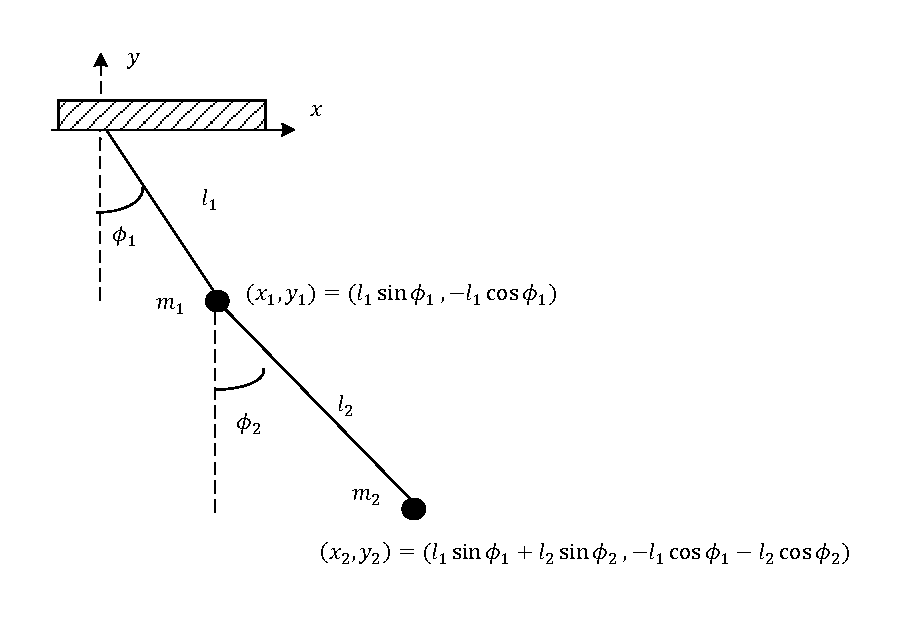
\includegraphics [width=10cm, height=8cm] {DoublePendulum}}
\caption{Pendulu bikoitza.}
\label{fig:41}
\end{figure} 

\subsubsection{Ekuazioak.}

\paragraph*{Hamiltondarra.}

\begin{equation*}
q=(\Theta_1,\Theta_2) \ \ , \ \ p=(P_1,P_2) \ \ , 
\end{equation*}

\begin{equation*} \label{eq:2}
H(q,p)= \bigg(\frac {C1 \ P_1^2 + C2 \ P_2^2 + 
 C3 \ P_1 \ P_2 \ \cos(\Theta_1 - \Theta_2)} {
 (C4 + C5 \ \sin^2 (Q_1 - Q_2))}\bigg)\\
       -C6 \ \cos(\Theta_1)-\ C7 \ \cos(\Theta_2), 
\end{equation*}

\paragraph*{}
     $C1 = l_2^2*m_2$,\\
     $C2 = l_1^2*(m_1 + m_2)$,\\
     $C3 = -2*l_1*l_2*l_2$,\\
     $C4 = 2*l_1^2*l_2^2*m_2*m_1$,\\
     $C5 = 2*m_1^2*l_2^2*m_2^2$,\\
     $C6 = g*l_1*(m_1 + m_2)$,\\
     $C7 = g*l_2*m_2$.


\paragraph*{Ekuazio diferentzialak.}

\begin{equation*}
\dot{\Theta_1}= \frac {2*C1*P1+C3*\cos(Q1-Q2)*P2}{aux1},
\end{equation*}

\begin{equation*}
 \ \ \dot{\Theta_2}= \frac{(2*C2*P2+C3*\cos(Q1-Q2)*P1)}{aux1},
\end{equation*}

\begin{equation*}
\dot{P1}=-(aux4+C6*\sin(Q1)), 
\end{equation*}

\begin{equation*}
\dot{P1}=(aux4-C7*\sin(Q2)), 
\end{equation*}

\paragraph*{}
$aux1=C4+C5*\sin(Q1-Q2)*\sin(Q1-Q2)$, \\
$aux2=C3*\cos(Q1-Q2)$,\\
$aux3=2*C5*\sin(Q1-Q2)*\cos(Q1-Q2)$,\\
$aux4=\frac{(-1/aux1^2)*(C1*P1^2+C2*P2^2+P1*P2*aux2)*aux3)-(C3*P1*P2*\sin(Q1-Q2))}{aux1}.$ 

\paragraph*{Jakobiarra.}
???

\subsubsection{Hasierako balioak.}

\paragraph*{\textbf{Sistemaren parametroak}.} 
Gure esperimentuetarako honako parametroak kontsideratuko ditugu,
\begin{equation*} \label{eq:17}
g=9.8 \ \frac{m}{sec^2}\,\ \ l_1=1.0 \ m \ , \ l_2=1.0 \ m\ , \ m_1=1.0 \ kg\ , \ m_2=1.0 \ kg
\end{equation*} 

\paragraph*{\textbf{Hasierako balioak}.}
Pendulu bikoitza konportamendu kaotikoa duen sistema ezlineala da. Zentzu honetan bi hasierako balio ezberdin kontsideratu ditugu \cite{Dumitru}:

\begin{enumerate}
   \item Hasierako balio ez-kaotikoak:   
   $q(0)=(1.1, 0)$ \ , \ $p(0)=(0,2.7746)$.
    
   \item Hasierako balio kaotikoak: \ \ \ \ \ \   
   $q(0)=(0,0)$ \ , \ \ \ \ $p(0)=(0,3.873)$.
\end{enumerate}


\subsubsection{Kodeak.}

Mathematican DoublePendulum.m paketean honako funtzioak inplementatu ditugu:

\begin{enumerate}
   \item Hamiltondarra: DoublePendulumHam.
   \item EDA: DoublePendulumODE.
   \item Jakobiarra: DoublePendulumJAC.
\end{enumerate}

\paragraph*{}C-lengoaian GaussUserProblem.c fitxategian honako funtzioak inplementatu ditugu:

\begin{enumerate}
   \item Hamiltondarra: HamPendulum().
   \item EDA: OdePendulum().
   \item Jakobiarra: JacPendulum().
\end{enumerate}

\subsection{N-Body problema.}

N gorputzeko problema grabitazionalari dagokionez, Eguzki sistemaren eredu sinplea integratuko dugu. Eguzki sistemaren gorputzak masa puntualak kontsideratuko ditugu eta gure ekuazio diferentzialek, gorputz hauen arteko erakarpen grabitazionalak bakarrik kontutan hartzen dituzte.Beraz, eguzki sistemaren eredu konplexuagoetako erlatibitate efektua, gorputzen formaren eragina, eta beste zenbait indar ez-grabitazionalak ez dira kontutan hartu.

$(N+1)$ gorputz kopurua izanik, $q_i,p_i\in \mathbb{R}^3, m_i \in \mathbb{R}$ gorputz bakoitzaren kokapena, momentua eta masa dira. Bestalde , momentua era honetan definituko dugu $p_i=m_i*v_i$ non $\frac{d q_i}{dt}=v_i$ den.


\subsubsection*{Equations.}

\paragraph*{Hamiltondarra.}

\begin{equation}
H(q,p)=\frac{1}{2}\ \sum^N_{i=0}{\ \frac{{\|p_i\|}^2}{m_i}}-G\ \sum^N_{0\le i<j\le N}{\frac{m_im_j}{\|q_i-q_j\|}} 
\end{equation}


\paragraph*{Ekuazio diferentzialak.}

\begin{equation}
\dot{q_i}=v_i, \  i=0,1,\dots N
\end{equation}

\begin{equation}
\dot{v_i}= \sum_{j=0,j \neq i}^{N} \frac{Gm_j}{\|q_j-q_i\|^3} (q_j-q_i)
\end{equation}

\paragraph{Jakobiarra.}

\begin{equation*}
\dot{y}=f(y)
\end{equation*}

\begin{equation}
Jac=\left(\begin{array}{cccccccc}
    \frac{\partial f_1}{\partial q_1} & \frac{\partial f_1}{\partial q_2} & \dots & \frac{\partial f_1}{\partial q_n} &
    \frac{\partial f_1}{\partial v_1} & \frac{\partial f_1}{\partial v_2} & \dots & \frac{\partial f_1}{\partial v_n}\\
    
    \dots & \dots & \dots & \dots & \dots & \dots & \dots & \dots \\
    
    \frac{\partial f_n}{\partial q_1} & \frac{\partial f_n}{\partial q_2} & \dots & \frac{\partial f_n}{\partial q_n} &
    \frac{\partial f_n}{\partial v_1} & \frac{\partial f_n}{\partial v_2} & \dots & \frac{\partial f_n}{\partial v_n}\\
  \end{array}\right)
\end{equation}

\paragraph*{}
And 2-body example,

\begin{equation}
J=\left(\begin{array}{cc}
  \ 0 & \ I \\
    A & \ 0 \\
\end{array}\right), \ \
Jac=\left(\begin{array}{ccccccccccccccc}
   & & q_{1x}  & q_{1y} & q_{1z}  & q_{2x}  & q_{2y} & q_{2z} & v_{1x}  & v_{1y} & v_{1z}  & v_{2x} & v_{2y} & v_{2z}  \\
   \\
   \frac{\partial f_1}{\partial q_{1x}} & & 0 & 0   & 0  & 0  & 0   & 0 & 1  &  0  & 0 & 0 & 0   & 0 \\
   \frac{\partial f_1}{\partial q_{1y}} & & 0 & 0   & 0  & 0  & 0   & 0 & 0  &  1  & 0 & 0 & 0   & 0 \\
   \frac{\partial f_1}{\partial q_{1z}} & & 0 & 0   & 0  & 0  & 0   & 0 & 0  &  0  & 1 & 0 & 0   & 0 \\
   \frac{\partial f_1}{\partial q_{2x}} & & 0 & 0   & 0  & 0  & 0   & 0 & 0  &  0  & 0 & 1 & 0   & 0 \\
   \frac{\partial f_1}{\partial q_{2y}} & & 0 & 0   & 0  & 0  & 0   & 0 & 0  &  0  & 0 & 0 & 1   & 0 \\
   \frac{\partial f_1}{\partial q_{2z}} & & 0 & 0   & 0  & 0  & 0   & 0 & 0  &  0  & 0 & 0 & 0   & 1 \\
   
   \frac{\partial f_1}{\partial v_{1x}} & & A & A   & A  & A  & A   & A & 0  &  0  & 0 & 0 & 0   & 0 \\
   \frac{\partial f_1}{\partial v_{1y}} & & A & A   & A  & A  & A   & A & 0  &  0  & 0 & 0 & 0   & 0 \\
   \frac{\partial f_1}{\partial v_{1z}} & & A & A   & A  & A  & A   & A & 0  &  0  & 0 & 0 & 0   & 0 \\
   \frac{\partial f_1}{\partial v_{2x}} & & A & A   & A  & A  & A   & A & 0  &  0  & 0 & 0 & 0   & 0 \\
   \frac{\partial f_1}{\partial v_{2y}} & & A & A   & A  & A  & A   & A & 0  &  0  & 0 & 0 & 0   & 0 \\
   \frac{\partial f_1}{\partial v_{2z}} & & A & A   & A  & A  & A   & A & 0  &  0  & 0 & 0 & 0   & 0 \\
  \end{array}\right)  
\end{equation}

\paragraph*{}Eta $A$ matrizearen deskribapena honako notazioaren laguntzaz,
\begin{equation*}
q_j-q_i=(x_{ji},y_{ji},z_{ji})
\end{equation*}
\begin{equation*}
\sum = \sum_{j=0,j \neq i}^{N}
\end{equation*}


\begin{enumerate}
\item $i==j$.\\
\begin{equation*}
A=\left(\begin{array}{ccc}
  \ \sum \bigg(\frac{3*Gm_j*x_{ji}^2}{\|q_j-q_i\|^5}\bigg)-
    \sum \bigg(\frac{Gm_j}{\|q_j-q_i\|^3} \bigg)& 
  \ \sum \bigg(\frac{3*Gm_j*(x_{ji}*y_{ji})}{\|q_j-q_i\|^5}\bigg)& 
  \ \sum \bigg(\frac{3*Gm_j*(x_{ij}*z_{ji})}{\|q_j-q_i\|^5}\bigg) \\
  
  \ \sum \bigg(\frac{3*Gm_j*(y_{ji}*x_{ji})}{\|q_j-q_i\|^5}\bigg)& 
  \ \sum \bigg(\frac{3*Gm_j*y_{ji}^2}{\|q_j-q_i\|^5}\bigg)-
          \sum \bigg(\frac{Gm_j}{\|q_j-q_i\|^3} \bigg)& 
    \ \sum \bigg(\frac{3*Gm_j*(y_{ji}*z_{ji})}{\|q_j-q_i\|^5}\bigg) \\
  
   \ \sum \bigg(\frac{3*Gm_j*(z_{ji}*x_{ji})}{\|q_j-q_i\|^5}\bigg)& 
   \ \sum \bigg(\frac{3*Gm_j*(z_{ji}*y_{ji})}{\|q_j-q_i\|^5}\bigg)& 
   \ \sum \bigg(\frac{3*Gm_j*z_{ji}^2}{\|q_j-q_i\|^5}\bigg)-
     \sum \bigg(\frac{Gm_j}{\|q_j-q_i\|^3} \bigg) \\
  
\end{array}\right)
\end{equation*}

\item $i \neq j$. \\
\begin{equation*}
A=\left(\begin{array}{ccc}
  \ \bigg(\frac{-3*Gm_j*x_{ji}^2}{\|q_j-q_i\|^5}\bigg)+
    \bigg(\frac{Gm_j}{\|q_j-q_i\|^3} \bigg)& 
  \ \bigg(\frac{-3*Gm_j*(x_{ji}*y_{ji})}{\|q_j-q_i\|^5}\bigg)& 
  \ \bigg(\frac{-3*Gm_j*(x_{ij}*z_{ji})}{\|q_j-q_i\|^5}\bigg) \\

  \ \bigg(\frac{-3*Gm_j*(y_{ji}*x_{ji})}{\|q_j-q_i\|^5}\bigg)& 
  \ \bigg(\frac{-3*Gm_j*y_{ji}^2}{\|q_j-q_i\|^5}\bigg)+
    \bigg(\frac{Gm_j}{\|q_j-q_i\|^3} \bigg)& 
  \ \bigg(\frac{-3*Gm_j*(y_{ji}*z_{ji})}{\|q_j-q_i\|^5}\bigg) \\
  
   \ \bigg(\frac{-3*Gm_j*(z_{ji}*x_{ji})}{\|q_j-q_i\|^5}\bigg)& 
   \ \bigg(\frac{-3*Gm_j*(z_{ji}*y_{ji})}{\|q_j-q_i\|^5}\bigg)& 
   \ \bigg(\frac{-3*Gm_j*z_{ji}^2}{\|q_j-q_i\|^5}\bigg)+
     \bigg(\frac{Gm_j}{\|q_j-q_i\|^3} \bigg) \\  
  
\end{array}\right)
\end{equation*}

\end{enumerate}

\subsubsection*{Hasierako balioak.}

The initial conditions and parameters have been taken from JPL Solar System ephemerids DE-405.
We have modified the velocities to get zero linear momentum.

\subsection{Inplementazioak.}

\paragraph*{} Mathematicako NBodyProblem.m paketean honako funtzioak garatu ditugu.

\begin{enumerate}
   \item Hamiltondarra: NBodyHAM.
   \item EDA: NBodyODE.
   \item Jakobiarra: Ez dut garatu.
\end{enumerate}

-\paragraph*{} C-lengoaiako inplementazioa:

\begin{enumerate}
   \item Hamiltondarra: HamNBody().
   \item EDA: OdeNbody().
   \item Jakobiarra: JacNBody().
\end{enumerate}



